%\begin{frame}{Opgave 6: Størrelsen af $N$}
%    Hvor stor skal $N$ være, for at fejlen er mindre end $10^{-10}$? 
%    Brug den oprindelige version af \textsc{Interpolation bin.py} til at sammenligne teori og numerisk eksperiment. 
%    Hvad er konklusionen? 
%    Hvor kommer problemerne fra? 
%    I den forbindelse kan I inddrage den grafiske undersøgelse fra punkt 4.
%\end{frame}

\begin{frame}{Størrelsen af $N$}
    Den teoretiske fejl (max) bliver $10^{-10}$ ved $N=48$, men i det numeriske eksperiment bliver fejlen aldrig mindre eller lig $10^{-10}$. 
    En mulig årsag til forandringer ved fejlen er divergens i yderpunkterne, hvilket kan gøre fejlen betydeligt større end den teoretiske, da de går mod $ \infty $ og $ - \infty $. Det kan også skyldes afrundingsfejl. 
    \begin{figure}
        \centering
            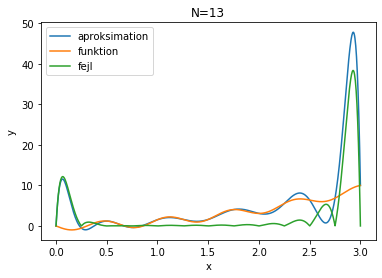
\includegraphics[scale=0.45]{images/N=13.png}.
    \end{figure}
\end{frame}